\pgfdeclareimage[width=\paperwidth,height=\paperheight]{bg}{imagenes/fondo_lab}
\setbeamertemplate{background}{\pgfuseimage{bg}}\subsection{Lab21: Filter taps}

%*********************
\begin{frame}{}

\pgfdeclareimage[width=\paperwidth,height=\paperheight]{bg}{imagenes/fondo_lab}
\setbeamertemplate{background}{\pgfuseimage{bg}}

\bfseries{\textrm{\LARGE Lab21\\ \Large Filter taps}}
\raggedright
\end{frame}
%*********************


\pgfdeclareimage[width=\paperwidth,height=\paperheight]{bg}{imagenes/fondo3}
\setbeamertemplate{background}{\pgfuseimage{bg}}
\begin{frame}{Filter taps}
Taps
\begin{flushleft}
El parámetro Taps indica las secciones de un filtro FIR el cual emula un retardo con múltiples trayectos. Uno de los parámetros mas importantes de este bloque son los coeficientes Taps pertenecientes al filtro. Uno de los beneficios de implementación del bloque es el poder definir el filtro acoplado directamente en este bloque, lo cual permitirá tener tanto el filtro acoplado como la corrección de tiempo de muestreo de manera simultánea. 
\end{flushleft}
\end{frame}

%*********************

\begin{frame}{Filter taps}
\begin{figure}[H]
\centering
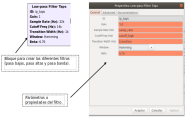
\includegraphics[width=.8\textwidth]{Modulaciones_digitales/lab21/pdf/lab21_1.pdf}
\end{figure}
\end{frame}
%*********************

\begin{frame}{Filter taps}
FIR Decimating
\begin{flushleft}
Este bloque permite cargar toques de filtro desde un archivo (herramienta de diseño de filtro). El nombre FIR proviene de la manera en la que el filtro afecta una señal.
Una función de impulso permite evidenciar que la señal es cero (0) siempre, excepto en algunos lugares donde se podrá observar que esta tendrá valor de uno (1). 
\end{flushleft}
\end{frame}

%*********************

\begin{frame}{Filter taps}
\begin{figure}[H]
\centering
\vspace{-3mm}
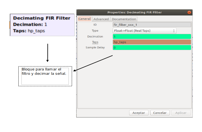
\includegraphics[width=\textwidth]{Modulaciones_digitales/lab21/pdf/lab21_2.pdf}
\end{figure}
\end{frame}

%*********************

\begin{frame}{Filter taps}
\begin{figure}[H]
\centering
\vspace{-3mm}
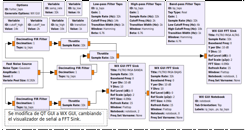
\includegraphics[width=\textwidth]{Modulaciones_digitales/lab21/pdf/lab21_3.pdf}
\end{figure}
\end{frame}
%*********************

\begin{frame}{Filter taps}
\begin{figure}[H]
\centering
\vspace{-3mm}
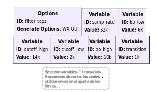
\includegraphics[width=\textwidth]{Modulaciones_digitales/lab21/pdf/lab21_4.pdf}
\end{figure}
\end{frame}

%*********************

\begin{frame}{Filter taps}
\begin{figure}[H]
\centering
\vspace{-3mm}
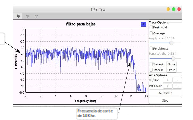
\includegraphics[width=\textwidth]{Modulaciones_digitales/lab21/pdf/lab21_5.pdf}
\end{figure}
\end{frame}

%*********************

\begin{frame}{Filter taps}
\begin{figure}[H]
\centering
\vspace{-3mm}
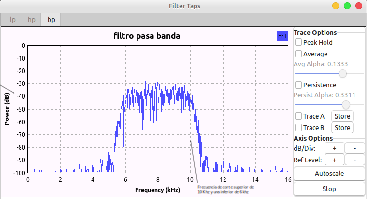
\includegraphics[width=\textwidth]{Modulaciones_digitales/lab21/pdf/lab21_6.pdf}
\end{figure}
\end{frame}
%*********************

\begin{frame}{Filter taps}
PASOS PARA OBTENER LA FRECUENCIA DE CORTE EN CADA FILTRO
\begin{flushleft}
1.	Lo primero que se debe tener en cuenta es el nivel máximo  (en dB’s) de la señal.\\
2.	Según la teoría la señal se encuentra a la mitad de su potencia cuando gráficamente este disminuye 3 dB’s.\\
3.	Se debe activar el rango de Average en el WX GUI FFT sink  con el valor mínimo.\\
4.	Seguido de eso podremos observar la frecuencia en la que se encuentra la señal en el momento de medir estos -3 dB’s.\\
5.	Tomar esa frecuencia como la frecuencia de corte inicial, final, o ambas según el filtro que se este utilizando. 
\end{flushleft}
\end{frame}

%*********************



